% Date : 01/11/2022
% Version : 1
% Auteur : Jimmy Roussel
% Relu : 
% Relecteur : 

% ------------------------------------------------------------ %
% ----------------------  Fiche ELC01  ----------------------- %
% Thème : Étude des circuits électriques I
% Classes : ???
% ------------------------------------------------------------ %



% ======================================================= % 
% ============== Gestion de la compilation ============== %
% ======================================================= % 
\ifdefined\mainIsLoaded\else
\RequirePackage{import}
\subimport{../../}{_preambule_CdE_PC}
\begin{document}
\fi
% ======================================================= % 
% ======================================================= % 






% ============================================================================ %
%                            FICHE D'ENTRAÎNEMENT                              %
% ============================================================================ %
% ======================= Métadonnées sur la fiche =========================== %
\titreFicheEntrainement		{Étude des circuits électriques I}
\grandTheme					{Électricité}
\numeroFiche				{ELC01}
\uniqueID					{eKdalRtYOdT} % une chaîne de caractères (a-z, A-Z) aléatoire de 10 caractères.
\nombreColonnesReponses		{3} % 1, 2, 3, etc.
% ============================================================================ %

%%%%%%%%%%%%%%%%%%%%%%%%%%%%%%%%%%%%%%%%%%%%%%%%%%%%%%%%%%%%%%%%%%%%%%%%%%%%%%%%%%%%%%%%%%%%%%
\debutFicheEntrainement                                                                      %
%%%%%%%%%%%%%%%%%%%%%%%%%%%%%%%%%%%%%%%%%%%%%%%%%%%%%%%%%%%%%%%%%%%%%%%%%%%%%%%%%%%%%%%%%%%%%%


% --------------------------------------------------------------------- %
%                              Prérequis                                %
%                             (facultatif)                              %
% --------------------------------------------------------------------- %
% ================== Métadonnées sur le prérequis ===================== %
\avecPrerequis{Y} % Y ou N
% ===================================================================== %
\begin{prerequis}
	Lois des n\oe uds. Loi des mailles. Loi d'Ohm. Montages diviseurs. %Pour les AN, on prendra :

\constantesUtiles
	\begin{listeConstantes}
		\item nombre d'Avogadro : $N_\text{A}=\np[mol^{-1}]{6.0e23}$
		\item charge élémentaire : $e=\np[C]{1.6e-19}$
	\end{listeConstantes}
\end{prerequis}
% --------------------------------------------------------------------- %









% •••••••••••••••••••••••••••••••••••••••••••••••••••••••••••••••••••••••••••• %
% •••••••••••••••••••••••••••••••••••••••••••••••••••••••••••••••••••••••••••• %
\sectionFicheEntrainement{Autour du courant électrique}
% •••••••••••••••••••••••••••••••••••••••••••••••••••••••••••••••••••••••••••• %
% •••••••••••••••••••••••••••••••••••••••••••••••••••••••••••••••••••••••••••• %






% ********************************************************************* %
%                           ENTRAÎNEMENT                                % 
% ********************************************************************* %
% ================ Métadonnées sur l'entraînement ===================== %
\titreEntrainementFacultatif	{Une bataille de courants}
\hauteurLargeurCadreReponse		{6mm}{1.5cm}
\dureeResolutionFacultative		{1} % 1, 2, 3 ou 4
\typeEntrainement				{QCM} % Newton ou QCM ou AN ou vide (exercice "normal")
\basiqueEtTransversal			{Y}
\nombreColonnesQuestions		{1} % vide, 1, 2, 3, etc.
\avecPlusieursQuestions			{N} % Y ou N
\initialisationEntrainement
% ===================================================================== %

% =============================================================================== %
\debutEntrainement
% =============================================================================== %

% ^^^^^^^^^^^^^^^^^^^^^^^^^^^^^^^^^^^^^^ %
%               Question                 %
% ^^^^^^^^^^^^^^^^^^^^^^^^^^^^^^^^^^^^^^ %
\begin{enonce}
Lequel de ces trois courants électriques présente la plus forte intensité ?
	
	\begin{listeQCM2Colonnes}
	\item \np{5000} électrons durant \np[ms]{1} 
	\item \np[mol]{.2} d'électrons durant \np[an]{1} 
	\item \np{20} milliards d'électrons durant \np[min]{1} 
	\end{listeQCM2Colonnes}
	\medskip
\end{enonce}

\reponse{\reponseB{}}

\begin{corrige}
	Calculons le nombre d'électrons transférés pendant une seconde : 
	\begin{itemize}
	\item \np{5000} électrons durant \np[ms]{1} correspond à $\np[s^{-1}]{5e6}$ ;
	\item \np[mol]{.2} d'électrons durant \np[an]{1} correspond à 
	\[
	\SI{.2}{mol}\times\np[mol^{-1}]{6.0e23}/\big(\SI{365}{jour.an^{-1}}\times \SI{24}{h.jour^{-1}}\times\SI{3600}{s.h^{-1}}\big)=\np[s^{-1}]{3.8e15}\; ;
	\] 
	\item \np{20} milliards d'électrons durant \np[min]{1} correspond à $\frac{\SI{20e9}{min^{-1}}}{\SI{60}{min/h^{-1}}}=\np[s^{-1}]{3.3e8}$.
	\end{itemize}
	Par conséquent, c'est le courant \reponseB{} qui donne la plus grande intensité.
\end{corrige}

% ************************************** %

% =============================================================================== %
\finEntrainement
% =============================================================================== %




% ********************************************************************* %
%                           ENTRAÎNEMENT                                % 
% ********************************************************************* %
% ================ Métadonnées sur l'entraînement ===================== %
\titreEntrainementFacultatif	{}%Un certain nombre}
\hauteurLargeurCadreReponse		{7mm}{2.5cm}
\dureeResolutionFacultative		{1} % 1, 2, 3 ou 4
\typeEntrainement				{AN} % Newton ou QCM ou AN ou vide (exercice "normal")
\basiqueEtTransversal			{Y}
\nombreColonnesQuestions		{1} % vide, 1, 2, 3, etc.
\avecPlusieursQuestions			{N} % Y ou N
\initialisationEntrainement
% ===================================================================== %

% =============================================================================== %
\debutEntrainement
% =============================================================================== %

L'intensité du courant traversant un fil de cuivre vaut $I=\np[mA]{4,0}$. 

% ^^^^^^^^^^^^^^^^^^^^^^^^^^^^^^^^^^^^^^ %
%               Question                 %
% ^^^^^^^^^^^^^^^^^^^^^^^^^^^^^^^^^^^^^^ %
\begin{enonce}
Combien d'électrons traversent la section du fil pendant \np[s]{10} ?
\end{enonce}

\reponse{\np{2.5e17}}

\begin{corrigeNewpage}
La quantité de charge transférée vaut $q=I\times \Delta t=\SI{4e-3}{A}\times \SI{10}{s}=\np[mC]{40}$. Cette quantité de charge correspond à un nombre d'électrons $N=q/e=\SI{40e-3}{C}/\SI{1.6e-19}{C}=\np{2.5e17}$ électrons.
\end{corrigeNewpage}


%La quantité de charge transférée vaut q = I × ∆t = 4 · 10−3 A × 10 s = 40 mC. Cette quantité de charge correspond à un nombre d’électrons N = q/e = 40 · 10−3 C/(1,6 · 10−19 C/e e) = 2,5 · 1017 électrons.

% ************************************** %

% =============================================================================== %
\finEntrainement
% =============================================================================== %




% ********************************************************************* %
%                           ENTRAÎNEMENT                                % 
% ********************************************************************* %
% ================ Métadonnées sur l'entraînement ===================== %

\titreEntrainementFacultatif	{Loi des n\oe uds}
\hauteurLargeurCadreReponse		{7mm}{3cm}
\dureeResolutionFacultative		{1} % 1, 2, 3 ou 4
\typeEntrainement				{Newton} % Newton ou QCM ou AN ou vide (exercice "normal")
\nombreColonnesQuestions		{1} % vide, 1, 2, 3, etc.
\avecPlusieursQuestions			{Y} % Y ou N
\initialisationEntrainement
% ===================================================================== %
% Un circuit électrique formé de 5 dipôles est représenté ci-contre. Certains courants algébriques sont indiqués. On cherche à compléter la figure.
\begin{center}
\subimport{_images/}{fiche_ELC01_loi_noeuds2_JRL_v1.tex}
\end{center}
Les courants indiqués sur le schéma ci-dessus sont algébriques.

En utilisant la loi des nœuds, déterminer en fonction de $i$ les courants suivants (on note $i_{\ptA\ptB}$ le courant qui va de A vers B, etc) :
% =============================================================================== %
\debutEntrainement
% =============================================================================== %


% ^^^^^^^^^^^^^^^^^^^^^^^^^^^^^^^^^^^^^^ %
%               Question                 %
% ^^^^^^^^^^^^^^^^^^^^^^^^^^^^^^^^^^^^^^ %

\begin{enonce}
$i_{\ptA\ptB}$
\end{enonce}

\reponse{$2i$}

%\begin{corrige}
%\end{corrige}
% ************************************** %

% ^^^^^^^^^^^^^^^^^^^^^^^^^^^^^^^^^^^^^^ %
%               Question                 %
% ^^^^^^^^^^^^^^^^^^^^^^^^^^^^^^^^^^^^^^ %

\begin{enonce}
$i_{\ptB\ptC}$
\end{enonce}

\reponse{$i$}

%\begin{corrige}
%\end{corrige}

% ************************************** %

% ^^^^^^^^^^^^^^^^^^^^^^^^^^^^^^^^^^^^^^ %
%               Question                 %
% ^^^^^^^^^^^^^^^^^^^^^^^^^^^^^^^^^^^^^^ %

\begin{enonce}
$i_{\ptC\ptD}$
\end{enonce}

\reponse{$0$}

%\begin{corrige}
%\end{corrige}

% ************************************** %

% =============================================================================== %
\finEntrainement
% =============================================================================== %


\newpage
% ********************************************************************* %
%                           ENTRAÎNEMENT                                % 
% ********************************************************************* %
% ================ Métadonnées sur l'entraînement ===================== %

\titreEntrainementFacultatif	{Loi des nœuds \emph{bis}}
\hauteurLargeurCadreReponse		{7mm}{20mm}
\dureeResolutionFacultative		{1} % 1, 2, 3 ou 4
\typeEntrainement				{AN} % Newton ou QCM ou AN ou vide (exercice "normal")
\nombreColonnesQuestions		{3} % vide, 1, 2, 3, etc.
\avecPlusieursQuestions			{Y} % Y ou N
\initialisationEntrainement
% ===================================================================== %


\begin{center}
\subimport{_images/}{fiche_ELC01_loi_noeuds1_CBD_v2.tex}
\end{center}

On considère le circuit électrique représenté ci-dessus. 

À partir de la loi des n\oe uds, calculer l'intensité des courants sans utiliser la calculatrice.

\medskip

%% mmmmmmmmmmmmmmmmmmmmmmmmmmmmmmmmmmmmmmmmmmmmmmmmmmmmmmmmm %
%% 		  Insertion d'une image en regard d'un texte
%% mmmmmmmmmmmmmmmmmmmmmmmmmmmmmmmmmmmmmmmmmmmmmmmmmmmmmmmmm %
%% --------------------------------------------------------- %
%\pourcentageDeLaPartieAGauche   {0.5}
%% --------------------------------------------------------- %
%%                                                           %
%% -------------------- Partie à gauche -------------------- %
%%                                                           %
%                                \initialisationPartieGauche % 
%%                                                           %
%%                                                           %
%On considère le circuit électrique représenté ci-contre. 
%
%\medskip
%
%À partir de la loi des n\oe uds, calculer l'intensité des courants sans utiliser la calculatrice.
%% --------------------------------------------------------- %
%%                                                           %
%% -------------------- Partie à droite -------------------- %
%%                                                           %
%                                \initialisationPartieDroite %
%%                                                           %
%%                                                           %
%\begin{center}
%\subimport{_images/}{fiche_ELC01_loi_noeuds1_JRL_v1.tex}
%\end{center}
%% --------------------------------------------------------- %
%                               \finalisationDuPartageDePage %					
%% --------------------------------------------------------- %
%
%\medskip
%\medskip

% =============================================================================== %
\debutEntrainement
% =============================================================================== %


% ^^^^^^^^^^^^^^^^^^^^^^^^^^^^^^^^^^^^^^ %
%               Question                 %
% ^^^^^^^^^^^^^^^^^^^^^^^^^^^^^^^^^^^^^^ %

\begin{enonce}
$i_1$
\end{enonce}

\reponse{$\np[mA]{80}$}

%\begin{corrige}
%\end{corrige}

% ************************************** %


% ^^^^^^^^^^^^^^^^^^^^^^^^^^^^^^^^^^^^^^ %
%               Question                 %
% ^^^^^^^^^^^^^^^^^^^^^^^^^^^^^^^^^^^^^^ %

\begin{enonce}
$i_2$
\end{enonce}

\reponse{$\np[mA]{30}$}

%\begin{corrige}
%\end{corrige}

% ************************************** %


% ^^^^^^^^^^^^^^^^^^^^^^^^^^^^^^^^^^^^^^ %
%               Question                 %
% ^^^^^^^^^^^^^^^^^^^^^^^^^^^^^^^^^^^^^^ %

\begin{enonce}
$i_3$
\end{enonce}

\reponse{$\np[mA]{-350}$}

%\begin{corrige}
%\end{corrige}

% ************************************** %

% =============================================================================== %
\finEntrainement
% =============================================================================== %

























% •••••••••••••••••••••••••••••••••••••••••••••••••••••••••••••••••••••••••••• %
% •••••••••••••••••••••••••••••••••••••••••••••••••••••••••••••••••••••••••••• %
\sectionFicheEntrainement{Autour de la tension électrique}
% •••••••••••••••••••••••••••••••••••••••••••••••••••••••••••••••••••••••••••• %
% •••••••••••••••••••••••••••••••••••••••••••••••••••••••••••••••••••••••••••• %




% ********************************************************************* %
%                           ENTRAÎNEMENT                                % 
% ********************************************************************* %
% ================ Métadonnées sur l'entraînement ===================== %

\titreEntrainementFacultatif	{Loi des mailles}
\hauteurLargeurCadreReponse		{7mm}{30mm}
\dureeResolutionFacultative		{1} % 1, 2, 3 ou 4
\typeEntrainement				{} % Newton ou QCM ou AN ou vide (exercice "normal")
\nombreColonnesQuestions		{1} % vide, 1, 2, 3, etc.
\avecPlusieursQuestions			{Y} % Y ou N
\initialisationEntrainement
% ===================================================================== 

% mmmmmmmmmmmmmmmmmmmmmmmmmmmmmmmmmmmmmmmmmmmmmmmmmmmmmmmmm %
% 		  Insertion d'une image en regard d'un texte
% mmmmmmmmmmmmmmmmmmmmmmmmmmmmmmmmmmmmmmmmmmmmmmmmmmmmmmmmm %
% --------------------------------------------------------- %
\pourcentageDeLaPartieAGauche   {0.5}
% --------------------------------------------------------- %
%                                                           %
% -------------------- Partie à gauche -------------------- %
%                                                           %
                                \initialisationPartieGauche % 
%                                                           %
%                                                           %
Un circuit électrique est formé d'une pile de f.é.m $E$ et de quatre dipôles. Certaines tensions sont indiquées.

À partir de la loi des mailles, exprimer en fonction de $E$ et $U_1$ les tensions suivantes:
% --------------------------------------------------------- %
%                                                           %
% -------------------- Partie à droite -------------------- %
%                                                           %
                                \initialisationPartieDroite %
%                                                           %
%                                                           %
\begin{center}
\subimport{_images/}{fiche_ELC01_loi_mailles2_CBD_v2.tex}
\end{center}
% --------------------------------------------------------- %
                               \finalisationDuPartageDePage %					
% --------------------------------------------------------- %

\medskip
% =============================================================================== %
\debutEntrainement
% =============================================================================== %

% ^^^^^^^^^^^^^^^^^^^^^^^^^^^^^^^^^^^^^^ %
%               Question                 %
% ^^^^^^^^^^^^^^^^^^^^^^^^^^^^^^^^^^^^^^ %

\begin{enonce}
$U$
\end{enonce}

\reponse{$E-U_1$}

\begin{corrige} 
	La loi des mailles donne la relation : $U+U_1-E=0$ soit $U=E-U_1$.
\end{corrige}

% ************************************** %


% ^^^^^^^^^^^^^^^^^^^^^^^^^^^^^^^^^^^^^^ %
%               Question                 %
% ^^^^^^^^^^^^^^^^^^^^^^^^^^^^^^^^^^^^^^ %

\begin{enonce}
$U_{\ptA\ptB}=V(\ptA)-V(\ptB)$
\end{enonce}

\reponse{$U_1-E$}

\begin{corrige}
	Les points \ptA et \ptC sont au même potentiel, ainsi que les points B et D. Par conséquent, la tension $U_{\ptA\ptB}=U_{\ptC\ptD}=-U_{\ptD\ptC}=-U$. Donc, $U_{\ptA\ptB}=U_1-E$.
\end{corrige}

% ************************************** %


% ^^^^^^^^^^^^^^^^^^^^^^^^^^^^^^^^^^^^^^ %
%               Question                 %
% ^^^^^^^^^^^^^^^^^^^^^^^^^^^^^^^^^^^^^^ %

\begin{enonce}
$U_{\ptD\ptA}$
\end{enonce}

\reponse{$E-U_1$}

\begin{corrige}
	\ptD est au même potentiel que \ptB de sorte que $U_{\ptD\ptA}=U_{\ptB\ptA}=-U_{\ptA\ptB}$. On trouve donc $U_{\ptD\ptA}=E-U_1$.
\end{corrige}

% ************************************** %

% =============================================================================== %
\finEntrainement
% =============================================================================== %


% ********************************************************************* %
%                           ENTRAÎNEMENT                                % 
% ********************************************************************* %
% ================ Métadonnées sur l'entraînement ===================== %

\titreEntrainementFacultatif	{Calculer une tension}
\hauteurLargeurCadreReponse		{7mm}{40mm}
\dureeResolutionFacultative		{1} % 1, 2, 3 ou 4
\typeEntrainement				{AN} % Newton ou QCM ou AN ou vide (exercice "normal")
\nombreColonnesQuestions		{1} % vide, 1, 2, 3, etc.
\avecPlusieursQuestions			{Y} % Y ou N
\initialisationEntrainement
% ===================================================================== %


% mmmmmmmmmmmmmmmmmmmmmmmmmmmmmmmmmmmmmmmmmmmmmmmmmmmmmmmmm %
% 		  Insertion d'une image en regard d'un texte
% mmmmmmmmmmmmmmmmmmmmmmmmmmmmmmmmmmmmmmmmmmmmmmmmmmmmmmmmm %
% --------------------------------------------------------- %
\pourcentageDeLaPartieAGauche   {0.5}
% --------------------------------------------------------- %
%                                                           %
% -------------------- Partie à gauche -------------------- %
%                                                           %
                                \initialisationPartieGauche % 
%                                                           %
%                                                           %
On considère le circuit électrique formé de deux sources idéales de tension et de quatre dipôles, comme représenté ci-contre. 

\smallskip

À partir de la loi des mailles, calculer les tensions :

% --------------------------------------------------------- %
%                                                           %
% -------------------- Partie à droite -------------------- %
%                                                           %
                                \initialisationPartieDroite %
%                                                           %
%                                                           %
\begin{center}
\subimport{_images/}{fiche_ELC01_loi_mailles1_JRL_v2.tex}
\end{center}
% --------------------------------------------------------- %
                               \finalisationDuPartageDePage %					
% --------------------------------------------------------- %

\bigskip
% =============================================================================== %
\debutEntrainement
% =============================================================================== %


% ^^^^^^^^^^^^^^^^^^^^^^^^^^^^^^^^^^^^^^ %
%               Question                 %
% ^^^^^^^^^^^^^^^^^^^^^^^^^^^^^^^^^^^^^^ %

\begin{enonce}
$U_1$
\end{enonce}

\reponse{\np[V]{1}}

\begin{corrige}
	Dans la maille triangulaire, on a $6=U_1+5$, soit $U_1=\np[V]{1}$.
\end{corrige}

% ************************************** %


% ^^^^^^^^^^^^^^^^^^^^^^^^^^^^^^^^^^^^^^ %
%               Question                 %
% ^^^^^^^^^^^^^^^^^^^^^^^^^^^^^^^^^^^^^^ %

\begin{enonce}
$U_2$
\end{enonce}

\reponse{\np[V]{-6}}

\begin{corrige}
	Dans la grande maille rectangulaire, la loi des mailles donne $12+U_2-6=0$, soit $U_2=\np[V]{-6}$.
\end{corrige}

% ************************************** %


% ^^^^^^^^^^^^^^^^^^^^^^^^^^^^^^^^^^^^^^ %
%               Question                 %
% ^^^^^^^^^^^^^^^^^^^^^^^^^^^^^^^^^^^^^^ %

\begin{enonce}
$U_3$
\end{enonce}

\reponse{\np[V]{7}}

\begin{corrige}
\minusMedskip
\minusBigskip

	\begin{center}
	%\subimport{_images/}{fiche_ELC01_loi_mailles1_q3_JRL_v2.tex}
	\begin{tikzpicture}[
	font=\footnotesize,
	maille/.style={ultra thick,\redOrBlack,postaction={decorate},decoration={markings,mark=at position 25mm with {\arrow[\redOrBlack]{stealth};},mark=at position 55mm with {\arrow[\redOrBlack]{stealth};}}},
	]
	\draw (0,-1)rectangle(4.5,1);
	\draw (4.5,1)--(3,0)--(4.5,-1);
	\draw (3,0)-|(1,1);
%	\pileL{}{};
	\FEMVL{}{12\,V};
	\FEMVR{shift={(4.5,0)}}{6\,V};
%	\pileR{shift={(4.5,0)}}{6\,V};
	\resistanceH{shift={(3.75,0.5)},rotate=33.7}{};
	\resistanceH{shift={(3.75,-0.5)},rotate=-33.7}{};
	\resistanceH{shift={(2,1)}}{};
	\resistanceH{shift={(2,0)}}{};
%	\draw[->,shift={(-.5,0)}](0,-.5)--++(0,1)node[midway,left=3pt]{\np[V]{12}};
	\draw[->,shift={(3.75,.5)},rotate=33.7](-.5,6pt)--++(1,0)node[pos=.7,left=3pt]{$U_1$};
	\draw[->,shift={(2,0.75)}](-0.5,0)--++(1,0)node[midway,below]{$U_2$};
	\draw[->,shift={(2,-.25)}](0.5,0)--++(-1,0)node[midway,below]{$U_3$};
	\draw[->,shift={(3.75,-.5)},rotate=-33.7](0.5,-6pt)--++(-1,0)node[pos=.3,left=3pt]{5\,V};
	\draw[maille](0,-1)|-(1,1)|-(3,0)--(4.5,-1)--cycle;
\end{tikzpicture}
	\end{center}
	
	Dans la maille surlignée et parcourue dans le sens indiqué, on trouve la relation $12-U_3-5=0$, ce qui donne $U_3=\np[V]{7}$. 
\end{corrige}

% ************************************** %

% =============================================================================== %
\finEntrainement
% =============================================================================== %























% •••••••••••••••••••••••••••••••••••••••••••••••••••••••••••••••••••••••••••• %
% •••••••••••••••••••••••••••••••••••••••••••••••••••••••••••••••••••••••••••• %
\newpage
\sectionFicheEntrainement{Loi d'Ohm}
% •••••••••••••••••••••••••••••••••••••••••••••••••••••••••••••••••••••••••••• %
% •••••••••••••••••••••••••••••••••••••••••••••••••••••••••••••••••••••••••••• %



% ********************************************************************* %
%                           ENTRAÎNEMENT                                % 
% ********************************************************************* %
% ================ Métadonnées sur l'entraînement ===================== %

\titreEntrainementFacultatif	{Caractéristiques}
\hauteurLargeurCadreReponse		{7mm}{40mm}
\dureeResolutionFacultative		{1} % 1, 2, 3 ou 4
\typeEntrainement				{Newton} % Newton ou QCM ou AN ou vide (exercice "normal")
\nombreColonnesQuestions		{1} % vide, 1, 2, 3, etc.
\avecPlusieursQuestions			{Y} % Y ou N
\initialisationEntrainement
% ===================================================================== %

On considère les cas suivants : 

\begin{center}
\subimport{_images/}{fiche_ELC01_loi_ohm_JRL_v2.tex}
\end{center}

Dans chaque cas, exprimer $i$ en fonction de $u$ et $R$.

\smallskip

% =============================================================================== %
\debutEntrainement
% =============================================================================== %


% ^^^^^^^^^^^^^^^^^^^^^^^^^^^^^^^^^^^^^^ %
%               Question                 %
% ^^^^^^^^^^^^^^^^^^^^^^^^^^^^^^^^^^^^^^ %

\begin{enonce}
Résistance 1
\end{enonce}

\reponse{$-\frac{u}{R}$}

\begin{corrige}
	La loi d'Ohm s'écrit $u=Ri$ en convention récepteur et $u=-Ri$ en convention générateur. Ici la résistance est fléchée en convention générateur. Ainsi, on trouve $i=-u/R$.
\end{corrige}

% ************************************** %


% ^^^^^^^^^^^^^^^^^^^^^^^^^^^^^^^^^^^^^^ %
%               Question                 %
% ^^^^^^^^^^^^^^^^^^^^^^^^^^^^^^^^^^^^^^ %

\begin{enonce}
Résistance 2
\end{enonce}

\reponse{$\frac{u}{2R}$}

\begin{corrige}
	La loi d'Ohm donne $u=2Ri$ soit $i=\frac{u}{2R}$.
\end{corrige}

% ************************************** %


% ^^^^^^^^^^^^^^^^^^^^^^^^^^^^^^^^^^^^^^ %
%               Question                 %
% ^^^^^^^^^^^^^^^^^^^^^^^^^^^^^^^^^^^^^^ %

\begin{enonce}
Résistance 3
\end{enonce}

\reponse{$\frac{u}{3R}$}

\begin{corrige}
	La résistance est fléchée en convention générateur : on a $u=-(3R)\times (-i)$, d'où $i=\frac{u}{3R}$.
\end{corrige}

% ************************************** %

% =============================================================================== %
\finEntrainement
% =============================================================================== %



% ********************************************************************* %
%                           ENTRAÎNEMENT                                % 
% ********************************************************************* %
% ================ Métadonnées sur l'entraînement ===================== %

\titreEntrainementFacultatif	{Résistances associées}
\hauteurLargeurCadreReponse		{10mm}{40mm}
\dureeResolutionFacultative		{3} % 1, 2, 3 ou 4
\typeEntrainement				{} % Newton ou QCM ou AN ou vide (exercice "normal")
\nombreColonnesQuestions		{1} % vide, 1, 2, 3, etc.
\avecPlusieursQuestions			{Y} % Y ou N
\initialisationEntrainement
% ===================================================================== %

Exprimer la résistance équivalente des dipôles AB suivants: 

% =============================================================================== %
\debutEntrainement
% =============================================================================== %

% ^^^^^^^^^^^^^^^^^^^^^^^^^^^^^^^^^^^^^^ %
%               Question                 %
% ^^^^^^^^^^^^^^^^^^^^^^^^^^^^^^^^^^^^^^ %

\begin{enonce}
\subimport{_images/}{ENT1.8a_JRL_v1.tex}
\end{enonce}

\reponse{$\frac56 R$}

\begin{corrige}
	$R_\text{eq}=\frac{R}{2}+\frac{R}{3}=\frac56 R$.
\end{corrige}
% ************************************** %

% ^^^^^^^^^^^^^^^^^^^^^^^^^^^^^^^^^^^^^^ %
%               Question                 %
% ^^^^^^^^^^^^^^^^^^^^^^^^^^^^^^^^^^^^^^ %

\begin{enonce}
\subimport{_images/}{ENT1.8b_JRL_v1.tex}
\end{enonce}

\reponse{$\frac{R}{5}$}

\begin{corrige}
	$\frac{1}{R_\text{eq}}=\frac{2}{R}+\frac{3}{R}=\frac{5}{R}$, soit $R_\text{eq}=\frac{R}{5}$.
\end{corrige}
% ************************************** %

% ^^^^^^^^^^^^^^^^^^^^^^^^^^^^^^^^^^^^^^ %
%               Question                 %
% ^^^^^^^^^^^^^^^^^^^^^^^^^^^^^^^^^^^^^^ %

\begin{enonce}
\subimport{_images/}{ENT1.8c_JRL_v1.tex}
\end{enonce}

\reponse{$\frac{R}{N}$}

\begin{corrige}
	$\frac{1}{R_\text{eq}}=\underbrace{\frac{1}{R}+\ldots+\frac{1}{R}}_{N\text{ fois}}=\frac{N}{R}$, d'où $R_\text{eq}=\frac{R}{N}$.	
\end{corrige}

% ************************************** %

% ^^^^^^^^^^^^^^^^^^^^^^^^^^^^^^^^^^^^^^ %
%               Question                 %
% ^^^^^^^^^^^^^^^^^^^^^^^^^^^^^^^^^^^^^^ %

\begin{enonce}
\subimport{_images/}{ENT1.8d_JRL_v1.tex}
\end{enonce}

\reponse{$R\left(\frac{1-a^2}{3-a^2}\right)$}

\begin{corrigeNewpage}
	La résistance équivalente $R_\text{eq}$ est telle que : 
	\[
	\frac{1}{R_\text{eq}}=\frac{1}{R}+\frac{1}{R(1+a)}+\frac{1}{R(1-a)}=
	\frac{1}{R}\left(1+\frac{1}{1+a}+\frac{1}{1-a}\right)=
	\frac{1}{R}\left(1+\frac{2}{1-a^2}\right)=
	\frac{1}{R}\left(\frac{3-a^2}{1-a^2}\right).
	\]
	On en déduit $R_\text{eq}=R\left(\frac{1-a^2}{3-a^2}\right)$.
\end{corrigeNewpage}

% ************************************** %
% % ^^^^^^^^^^^^^^^^^^^^^^^^^^^^^^^^^^^^^^ %
% %               Question                 %
% % ^^^^^^^^^^^^^^^^^^^^^^^^^^^^^^^^^^^^^^ %
%
% \begin{enonce}
% $N$ conducteurs en série, de résistances $R_1=R$, $R_2=2R,\ldots$, $R_N=NR$
% \end{enonce}
%
% \reponse{$\frac{N(N+1)}{2}R$}
%
% \begin{corrige}
% 	$R_\text{eq}=R+2R+\ldots+NR=R(\underbrace{1+2+\ldots+N}_{\frac{N(N+1)}{2}})=\frac{N(N+1)}{2}R$
% \end{corrige}
%
% % ************************************** %

% =============================================================================== %
\finEntrainement
% =============================================================================== %


\newpage
% ********************************************************************* %
%                           ENTRAÎNEMENT                                % 
% ********************************************************************* %
% ================ Métadonnées sur l'entraînement ===================== %

\titreEntrainementFacultatif	{Trois résistances équivalentes}
\hauteurLargeurCadreReponse		{7mm}{15mm}
\dureeResolutionFacultative		{1} % 1, 2, 3 ou 4
\typeEntrainement				{AN} % Newton ou QCM ou AN ou vide (exercice "normal")
\nombreColonnesQuestions		{3} % vide, 1, 2, 3, etc.
\avecPlusieursQuestions			{Y} % Y ou N
\initialisationEntrainement
% ===================================================================== %


% Les trois dipôles électriques suivants sont équivalents à un conducteur ohmique.
\begin{center}
\subimport{_images/}{fiche_ELC01_Req1_CBD_v2.tex}
\end{center}

Sans utiliser la calculatrice, calculer la résistance équivalente

% =============================================================================== %
\debutEntrainement
% =============================================================================== %


% ^^^^^^^^^^^^^^^^^^^^^^^^^^^^^^^^^^^^^^ %
%               Question                 %
% ^^^^^^^^^^^^^^^^^^^^^^^^^^^^^^^^^^^^^^ %

\begin{enonce}
du dipôle 1
\end{enonce}

\reponse{\np[k\Omega]{1}}

\begin{corrige}
	En associant les deux résistances en série, on se ramène à deux résistances de \np[k\Omega]{2} en parallèle, ce qui est équivalent à une résistance de \np[k\Omega]{1}.
\end{corrige}

% ************************************** %


% ^^^^^^^^^^^^^^^^^^^^^^^^^^^^^^^^^^^^^^ %
%               Question                 %
% ^^^^^^^^^^^^^^^^^^^^^^^^^^^^^^^^^^^^^^ %

\begin{enonce}
du dipôle 2
\end{enonce}

\reponse{\np[k\Omega]{1}}

\begin{corrige}
	En répétant la méthode précédente plusieurs fois, on arrive au même résultat.
\end{corrige}

% ************************************** %


% ^^^^^^^^^^^^^^^^^^^^^^^^^^^^^^^^^^^^^^ %
%               Question                 %
% ^^^^^^^^^^^^^^^^^^^^^^^^^^^^^^^^^^^^^^ %

\begin{enonce}
du dipôle 3
\end{enonce}

\reponse{\np[k\Omega]{1}}

%\begin{corrige}
%\end{corrige}

% ************************************** %

% =============================================================================== %
\finEntrainement


% =============================================================================== %
% ********************************************************************* %
%                           ENTRAÎNEMENT                                % 
% ********************************************************************* %
% ================ Métadonnées sur l'entraînement ===================== %

\titreEntrainementFacultatif	{Une autre résistance équivalente}
\hauteurLargeurCadreReponse		{10mm}{25mm}
\dureeResolutionFacultative		{2} % 1, 2, 3 ou 4
\typeEntrainement				{} % Newton ou QCM ou AN ou vide (exercice "normal")
\nombreColonnesQuestions		{1} % vide, 1, 2, 3, etc.
\avecPlusieursQuestions			{N} % Y ou N
\initialisationEntrainement
% ===================================================================== %

% mmmmmmmmmmmmmmmmmmmmmmmmmmmmmmmmmmmmmmmmmmmmmmmmmmmmmmmmm %
% 		  Insertion d'une image en regard d'un texte
% mmmmmmmmmmmmmmmmmmmmmmmmmmmmmmmmmmmmmmmmmmmmmmmmmmmmmmmmm %
% --------------------------------------------------------- %
\pourcentageDeLaPartieAGauche   {0.5}
% --------------------------------------------------------- %
%                                                           %
% -------------------- Partie à gauche -------------------- %
%                                                           %
                                \initialisationPartieGauche % 
%                                                           %
%                                                           %
On considère le dipôle AB constitué uniquement de conducteurs ohmiques.  

\medskip

% --------------------------------------------------------- %
%                                                           %
% -------------------- Partie à droite -------------------- %
%                                                           %
                                \initialisationPartieDroite %
%                                                           %
%                                                           %
\begin{center}
\subimport{_images/}{fiche_ELC01_Req2_JRL_v1.tex}
\end{center}
% --------------------------------------------------------- %
                               \finalisationDuPartageDePage %					
% --------------------------------------------------------- %

\medskip

% =============================================================================== %
\debutEntrainement
% =============================================================================== %
% ^^^^^^^^^^^^^^^^^^^^^^^^^^^^^^^^^^^^^^ %
%               Question                 %
% ^^^^^^^^^^^^^^^^^^^^^^^^^^^^^^^^^^^^^^ %

\begin{enonce}
Exprimer la résistance équivalente du dipôle AB en fonction de $R$ et $R'$.
\end{enonce}

\reponse{$\frac{4R(R+R')}{2R+R'}$}

\begin{corrige}
	La résistance équivalente du dipôle AB vaut $R_\text{eq}=2R+\frac{2RR'}{2R+R'}$ soit $R_\text{eq}=\frac{4R(R+R')}{2R+R'}$.
\end{corrige}

% =============================================================================== %
\finEntrainement
% =============================================================================== %



% ********************************************************************* %
%                           ENTRAÎNEMENT                                % 
% ********************************************************************* %
% ================ Métadonnées sur l'entraînement ===================== %

\pointInterrogation				{Y}
\titreEntrainementFacultatif	{Quelle résistance choisir}
\hauteurLargeurCadreReponse		{7mm}{15mm}
\dureeResolutionFacultative		{3} % 1, 2, 3 ou 4
\typeEntrainement				{} % Newton ou QCM ou AN ou vide (exercice "normal")
\basiqueEtTransversal			{Y}
\nombreColonnesQuestions		{3} % vide, 1, 2, 3, etc.
\avecPlusieursQuestions			{Y} % Y ou N
\initialisationEntrainement
% ===================================================================== %

La résistance équivalente d'un dipôle s'écrit 
\[
R_\text{eq}=\frac{4R(R+R')}{2R+R'}.
\]
Déterminer la valeur de $R'$ pour que %si l'on veut que le dipôle soit équivalent à un conducteur ohmique de résistance :
% =============================================================================== %
\debutEntrainement
% =============================================================================== %
% ^^^^^^^^^^^^^^^^^^^^^^^^^^^^^^^^^^^^^^ %
%               Question                 %
% ^^^^^^^^^^^^^^^^^^^^^^^^^^^^^^^^^^^^^^ %

\begin{enonce}
$R_\text{eq} = 3R$
\end{enonce}

\reponse{$2R$}

\begin{corrige}
On doit résoudre 
\[
\frac{4R(R+R')}{2R+R'}=3R
\quad\text{soit}\quad
4R^2+4RR'=6R^2+3RR'
\quad\text{d'où}\quad
RR'=2R^2.
\]
Comme $R\neq 0$, on obtient $R'=2R$.
\end{corrige}

% ************************************** %


% ^^^^^^^^^^^^^^^^^^^^^^^^^^^^^^^^^^^^^^ %
%               Question                 %
% ^^^^^^^^^^^^^^^^^^^^^^^^^^^^^^^^^^^^^^ %

\begin{enonce}
$R_\text{eq} = \frac{8}{3}R$
\end{enonce}

\reponse{$R$}

\begin{corrige}
On doit résoudre 
\[
\frac{4R(R+R')}{2R+R'}=\frac83 R
\quad\text{soit}\quad
12R^2+12RR'=16R^2+8RR'
\quad\text{d'où}\quad
4RR'=4R^2.
\]
Comme $R\neq 0$, on obtient $R'=R$.
\end{corrige}

% ************************************** %


% ^^^^^^^^^^^^^^^^^^^^^^^^^^^^^^^^^^^^^^ %
%               Question                 %
% ^^^^^^^^^^^^^^^^^^^^^^^^^^^^^^^^^^^^^^ %

\begin{enonce}
$R_\text{eq} = 2R$
\end{enonce}

\reponse{$0$}

\begin{corrige}
Résolvons l'équation 
\[
\frac{4R(R+R')}{2R+R'}=2 R
\quad\text{soit}\quad
4R^2+4RR'=4R^2+2RR'
\quad\text{d'où}\quad
2RR'=0.
\]
Comme $R\neq 0$, il faut nécessairement $R'=0$.
\end{corrige}

% ************************************** %

% =============================================================================== %
\finEntrainement
% =============================================================================== %













% •••••••••••••••••••••••••••••••••••••••••••••••••••••••••••••••••••••••••••• %
% •••••••••••••••••••••••••••••••••••••••••••••••••••••••••••••••••••••••••••• %
\sectionFicheEntrainement{Résoudre une équation électrique}
% •••••••••••••••••••••••••••••••••••••••••••••••••••••••••••••••••••••••••••• %
% •••••••••••••••••••••••••••••••••••••••••••••••••••••••••••••••••••••••••••• %





% ********************************************************************* %
%                           ENTRAÎNEMENT                                % 
% ********************************************************************* %
% ================ Métadonnées sur l'entraînement ===================== %

\titreEntrainementFacultatif	{Une équation de maille}
\hauteurLargeurCadreReponse		{7mm}{50mm}
\dureeResolutionFacultative		{1} % 1, 2, 3 ou 4
\typeEntrainement				{Newton} % Newton ou QCM ou AN ou vide (exercice "normal")
\basiqueEtTransversal			{Y}
\nombreColonnesQuestions		{1} % vide, 1, 2, 3, etc.
\avecPlusieursQuestions			{Y} % Y ou N
\initialisationEntrainement
% ===================================================================== %

Dans un circuit, la loi des mailles se traduit par la relation $R_1I+R_2(I_0+I)=2R_2 I_0$.

% =============================================================================== %
\debutEntrainement
% =============================================================================== %

% ^^^^^^^^^^^^^^^^^^^^^^^^^^^^^^^^^^^^^^ %
%               Question                 %
% ^^^^^^^^^^^^^^^^^^^^^^^^^^^^^^^^^^^^^^ %

\begin{enonce}
	On suppose que $R_1 = 2R_2$. Exprimer $I$ en fonction de $I_0$
\end{enonce}

\reponse{$\frac{I_0}{3}$}

%\begin{corrige}
%
%\end{corrige}

% ************************************** %

% ^^^^^^^^^^^^^^^^^^^^^^^^^^^^^^^^^^^^^^ %
%               Question                 %
% ^^^^^^^^^^^^^^^^^^^^^^^^^^^^^^^^^^^^^^ %

\begin{enonce}
	Exprimer $I$ en fonction de $R_1$, $R_2$ et $I_0$
\end{enonce}

\reponse{$\frac{R_2}{R_1+R_2}I_0$}

\begin{corrige}
	Isolons $I$ : \minusSmallskip
	\[
		\begin{array}{rcl}
			R_1I+R_2(I_0+I)		&=&2R_2 I_0		\\
			(R_1+R_2)I+R_2I_0	&=&2R_2 I_0		\\
			(R_1+R_2)I			&=&R_2 I_0		\\
			I					&=&\frac{R_2}{R_1+R_2}I_0.
		\end{array}
	\]	
	
\end{corrige}

% ************************************** %



% =============================================================================== %
\finEntrainement
% =============================================================================== %

\newpage





% ********************************************************************* %
%                           ENTRAÎNEMENT                                % 
% ********************************************************************* %
% ================ Métadonnées sur l'entraînement ===================== %

\titreEntrainementFacultatif	{Circuit à 2 mailles}
\hauteurLargeurCadreReponse		{7mm}{50mm}
\dureeResolutionFacultative		{2} % 1, 2, 3 ou 4
\typeEntrainement				{} % Newton ou QCM ou AN ou vide (exercice "normal")
\nombreColonnesQuestions		{2} % vide, 1, 2, 3, etc.
\avecPlusieursQuestions			{Y} % Y ou N
\initialisationEntrainement
% ===================================================================== %


% mmmmmmmmmmmmmmmmmmmmmmmmmmmmmmmmmmmmmmmmmmmmmmmmmmmmmmmmm %
% 		  Insertion d'une image en regard d'un texte
% mmmmmmmmmmmmmmmmmmmmmmmmmmmmmmmmmmmmmmmmmmmmmmmmmmmmmmmmm %
% --------------------------------------------------------- %
\pourcentageDeLaPartieAGauche   {0.5}
% --------------------------------------------------------- %
%                                                           %
% -------------------- Partie à gauche -------------------- %
%                                                           %
                                \initialisationPartieGauche % 
%                                                           %
%                                                           %
On forme un circuit avec une pile et trois conducteurs ohmiques. On définit les courants algébriques $i$ et $i_1$ comme indiqué ci-contre. 

\medskip

Exprimer $E$ en fonction de $i$, $i_1$ et $R$ en appliquant la loi des mailles dans la maille :
% --------------------------------------------------------- %
%                                                           %
% -------------------- Partie à droite -------------------- %
%                                                           %
                                \initialisationPartieDroite %
%                                                           %
%                                                           %
\begin{center}
\subimport{_images/}{fiche_ELC01_loi_mailles3_CBD_v2.tex}
\end{center}
% --------------------------------------------------------- %
                               \finalisationDuPartageDePage %					
% --------------------------------------------------------- %

\medskip
% =============================================================================== %
\debutEntrainement
% =============================================================================== %


% ^^^^^^^^^^^^^^^^^^^^^^^^^^^^^^^^^^^^^^ %
%               Question                 %
% ^^^^^^^^^^^^^^^^^^^^^^^^^^^^^^^^^^^^^^ %

\begin{enonce}
(ABCF)
\end{enonce}

\reponse{$\frac14 Ri+Ri_1$}

\begin{corrige} 
	Appliquons la loi des mailles en parcourant la maille dans le sens ABCF : 
	\[
	E-\frac14 Ri-Ri_1=0
	\quad\text{soit}\quad
	E=\frac14 Ri+Ri_1.
	\]
\end{corrige}

% ************************************** %


% ^^^^^^^^^^^^^^^^^^^^^^^^^^^^^^^^^^^^^^ %
%               Question                 %
% ^^^^^^^^^^^^^^^^^^^^^^^^^^^^^^^^^^^^^^ %

\begin{enonce}
(ABDE)
\end{enonce}

\reponse{$\frac{13}{4}Ri-3Ri_1$}

\begin{corrigeNewpage}
	Appliquons la loi des mailles en parcourant la maille dans le sens ABDE : 
	\[
	E-\frac14 Ri-3R(i-i_1)=0
	\quad\text{d'où}\quad
	E=\frac{13}{4}Ri-3Ri_1.
	\]
\end{corrigeNewpage}

% ************************************** %

% =============================================================================== %
\finEntrainement
% =============================================================================== %






% ********************************************************************* %
%                           ENTRAÎNEMENT                                % 
% ********************************************************************* %
% ================ Métadonnées sur l'entraînement ===================== %

\titreEntrainementFacultatif	{}
\hauteurLargeurCadreReponse		{9mm}{35mm}
\dureeResolutionFacultative		{2} % 1, 2, 3 ou 4
\typeEntrainement				{Newton} % Newton ou QCM ou AN ou vide (exercice "normal")
\basiqueEtTransversal			{Y}
\nombreColonnesQuestions		{1} % vide, 1, 2, 3, etc.
\avecPlusieursQuestions			{Y} % Y ou N
\initialisationEntrainement
% ===================================================================== %

Dans l'entraînement précédent, les grandeurs $i$ et $i_1$ vérifient le système $\systeme{Ri+4Ri_1=4E,13Ri-12Ri_1=4E}$

\smallskip

% =============================================================================== %
\debutEntrainement
% =============================================================================== %

% ^^^^^^^^^^^^^^^^^^^^^^^^^^^^^^^^^^^^^^ %
%               Question                 %
% ^^^^^^^^^^^^^^^^^^^^^^^^^^^^^^^^^^^^^^ %

\begin{enonce}
Déterminer $i$ en fonction de $E$  et $R$.
\end{enonce}

\reponse{$\frac{E}{R}$}

\begin{corrige}
	Additionnons les deux relations après avoir multiplié par 3 la première
	\[
	\systeme{3Ri+12Ri_1=12E,13Ri-12Ri_1=4E}
	\quad\text{ donnent ainsi }\quad
	16 Ri=16E	
	\quad\text{d'où}\quad
	i=\frac{E}{R}.
	\]
\end{corrige}

% ^^^^^^^^^^^^^^^^^^^^^^^^^^^^^^^^^^^^^^ %
%               Question                 %
% ^^^^^^^^^^^^^^^^^^^^^^^^^^^^^^^^^^^^^^ %

\begin{enonce}
	Déterminer $i_1$ en fonction de $E$ et $R$.	
\end{enonce}

\reponse{$\frac{3E}{4R}$}

\begin{corrige}
	Dans la première relation, remplaçons $i$ par $E/R$ :
	\[
	R\times\left(\frac{E}{R}\right)+4Ri_1=4E
	\quad\text{ donc }\quad
	4Ri_1=3E	
	\quad\text{d'où}\quad
	i_1=\frac{3E}{4R}.
	\]
\end{corrige}

% ************************************** %

% =============================================================================== %
\finEntrainement
% =============================================================================== %









% •••••••••••••••••••••••••••••••••••••••••••••••••••••••••••••••••••••••••••• %
% •••••••••••••••••••••••••••••••••••••••••••••••••••••••••••••••••••••••••••• %
\sectionFicheEntrainement{Diviseurs}
% •••••••••••••••••••••••••••••••••••••••••••••••••••••••••••••••••••••••••••• %
% •••••••••••••••••••••••••••••••••••••••••••••••••••••••••••••••••••••••••••• %


% ********************************************************************* %
%                           ENTRAÎNEMENT                                % 
% ********************************************************************* %
% ================ Métadonnées sur l'entraînement ===================== %
\titreEntrainementFacultatif	{Un diviseur de tension}
\hauteurLargeurCadreReponse		{10mm}{30mm}
\dureeResolutionFacultative		{2} % 1, 2, 3 ou 4
\typeEntrainement				{} % Newton ou QCM ou AN ou vide (exercice "normal")
\nombreColonnesQuestions		{3} % vide, 1, 2, 3, etc.
\avecPlusieursQuestions			{Y} % Y ou N
\initialisationEntrainement
% ===================================================================== 

% mmmmmmmmmmmmmmmmmmmmmmmmmmmmmmmmmmmmmmmmmmmmmmmmmmmmmmmmm %
% 		  Insertion d'une image en regard d'un texte
% mmmmmmmmmmmmmmmmmmmmmmmmmmmmmmmmmmmmmmmmmmmmmmmmmmmmmmmmm %
% --------------------------------------------------------- %
\pourcentageDeLaPartieAGauche   {0.6}
% --------------------------------------------------------- %
%                                                           %
% -------------------- Partie à gauche -------------------- %
%                                                           %
                                \initialisationPartieGauche % 
%                                                           %
%                                                           %
On forme un circuit avec une pile de f.é.m $E$ et quatre conducteurs ohmiques. On définit les tensions $U_1$, $U_2$ et $U_3$ comme indiqué ci-contre. 

Exprimer en fonction de $E$, $R_1$, $R_2$, $R_3$ et $R_4$, les tensions :

\medskip

% --------------------------------------------------------- %
%                                                           %
% -------------------- Partie à droite -------------------- %
%                                                           %
                                \initialisationPartieDroite %
%                                                           %
%                                                           %
\begin{center}
\subimport{_images/}{ENT1.15_CBD_v2.tex}
\end{center}
% --------------------------------------------------------- %
                               \finalisationDuPartageDePage %					
% --------------------------------------------------------- %
\medskip
% =============================================================================== %
\debutEntrainement
% =============================================================================== %
% ^^^^^^^^^^^^^^^^^^^^^^^^^^^^^^^^^^^^^^ %
%               Question                 %
% ^^^^^^^^^^^^^^^^^^^^^^^^^^^^^^^^^^^^^^ %

\begin{enonce}
$U_1$
\end{enonce}

\reponse{$\frac{ER_1}{R_1+R_2+R_3+R_4}$}

\begin{corrige}
Rappelons la règle du diviseur de tension : 

Dans un circuit où $N$ conducteurs de résistances $R_1, \ldots, R_N$ sont placés en série, la tension $U_k$ qui règne aux bornes de la résistance $R_k$ est donnée par la formule 
$$
U_k=\frac{R_k}{R_1 + R_2 + \cdots + R_N}\, U
\quad\text{avec}\quad
U=\sum_{i=1}^N U_i.
$$
Ici, cela donne $U_1=E\times \frac{R_1}{R_1+R_2+R_3+R_4}$.
\end{corrige}
% ^^^^^^^^^^^^^^^^^^^^^^^^^^^^^^^^^^^^^^ %
%               Question                 %
% ^^^^^^^^^^^^^^^^^^^^^^^^^^^^^^^^^^^^^^ %

\begin{enonce}
$U_2$
\end{enonce}

\reponse{$\frac{E(R_2+R_3)}{R_1+R_2+R_3+R_4}$}

\begin{corrige}
Ici, on cherche la tension aux bornes de l'ensemble des résistances $\{R_2,R_3\}$ placés en série et donc équivalent à $R_2+R_3$. La règle du diviseur donne alors $U_2=E\times\frac{R_2+R_3}{R_1+R_2+R_3+R_4}$.

\end{corrige}
% ^^^^^^^^^^^^^^^^^^^^^^^^^^^^^^^^^^^^^^ %
%               Question                 %
% ^^^^^^^^^^^^^^^^^^^^^^^^^^^^^^^^^^^^^^ %

\begin{enonce}
$U_3$
\end{enonce}

\reponse{$\frac{-ER_4}{R_1+R_2+R_3+R_4}$}

\begin{corrige}
Attention, ici il y a un piège. La loi du diviseur de tension donne $U_3=U\frac{R_4}{R_1+R_2+R_3+R_4}$ où $U$ est la somme algébrique des tensions orientées dans le même sens que la tension que l'on cherche. Aussi a-t-on  $U=-E$ de sorte que $U_3=-E\times\frac{R_4}{R_1+R_2+R_3+R_4}$.
\end{corrige}



% =============================================================================== %
\finEntrainement
% =============================================================================== %







% ********************************************************************* %
%                           ENTRAÎNEMENT                                % 
% ********************************************************************* %
% ================ Métadonnées sur l'entraînement ===================== %

\titreEntrainementFacultatif	{Un diviseur de courant}
\hauteurLargeurCadreReponse		{7mm}{15mm}
\dureeResolutionFacultative		{2} % 1, 2, 3 ou 4
\typeEntrainement				{N} % Newton ou QCM ou AN ou vide (exercice "normal")
\nombreColonnesQuestions		{1} % vide, 1, 2, 3, etc.
\avecPlusieursQuestions			{Y} % Y ou N
\initialisationEntrainement
% ===================================================================== %

\begin{center}
\subimport{_images/}{fiche_ELC01_diviseur_courant2_JRL_v1.tex}
\end{center}

\minusSmallskip

% =============================================================================== %
\debutEntrainement
% =============================================================================== %

% ^^^^^^^^^^^^^^^^^^^^^^^^^^^^^^^^^^^^^^ %
%               Question                 %
% ^^^^^^^^^^^^^^^^^^^^^^^^^^^^^^^^^^^^^^ %

\begin{enonce}
Pour quelle valeur de $\alpha$, a-t-on $i_1=i/3$ ?
\end{enonce}

\reponse{$2$}

\begin{corrige}
La formule du diviseur de courant donne $\frac{i_1}{i}=\frac{1/(\alpha R)}{1/(\alpha R)+1/R}$. Par conséquent, $\alpha$ doit vérifier l'équation 
\[
	\frac{1}{1+\alpha}=\frac13
	\quad\text{c'est-à-dire}\quad
	\alpha=2.
\]
\end{corrige}
% ************************************** %
% ^^^^^^^^^^^^^^^^^^^^^^^^^^^^^^^^^^^^^^ %
%               Question                 %
% ^^^^^^^^^^^^^^^^^^^^^^^^^^^^^^^^^^^^^^ %

\begin{enonce}
Pour quelle valeur de $\alpha$, a-t-on $i_2=3 i_1$ ?
\end{enonce}

\reponse{$3$}

\begin{corrige}
On peut utiliser les formules du diviseur de courant : 
\[
	i_1=i\times\frac{1/(\alpha R)}{1/(\alpha R)+1/R}
	\quad\text{et}\quad
	i_2=i\times\frac{1/R}{1/(\alpha R)+1/R}
\]
ce qui permet de déduire $i_2/i_1=\alpha$. La solution est donc $\alpha=3$.

On peut aussi tout simplement écrire la loi des mailles : $\alpha R i_1=Ri_2$ pour aboutir plus immédiatement au résultat.
\end{corrige}
% ************************************** %

% =============================================================================== %
\finEntrainement



% ********************************************************************* %
%                           ENTRAÎNEMENT                                % 
% ********************************************************************* %
% ================ Métadonnées sur l'entraînement ===================== %
\titreEntrainementFacultatif	{Exercice de synthèse I}
\hauteurLargeurCadreReponse		{8mm}{25mm}
\dureeResolutionFacultative		{2} % 1, 2, 3 ou 4
\typeEntrainement				{} % Newton ou QCM ou AN ou vide (exercice "normal")
\nombreColonnesQuestions		{1} % vide, 1, 2, 3, etc.
\avecPlusieursQuestions			{Y} % Y ou N
\initialisationEntrainement
% ===================================================================== %
% mmmmmmmmmmmmmmmmmmmmmmmmmmmmmmmmmmmmmmmmmmmmmmmmmmmmmmmmm %
% 		  Insertion d'une image en regard d'un texte
% mmmmmmmmmmmmmmmmmmmmmmmmmmmmmmmmmmmmmmmmmmmmmmmmmmmmmmmmm %
% --------------------------------------------------------- %
\pourcentageDeLaPartieAGauche   {0.5}
% --------------------------------------------------------- %
%                                                           %
% -------------------- Partie à gauche -------------------- %
%                                                           %
                                \initialisationPartieGauche % 
%                                                           %
%                                                           %
On forme un circuit avec une pile et trois conducteurs ohmiques. On définit les tensions $U_1$ et $U_2$ comme indiqué ci-contre. 

\medskip

% --------------------------------------------------------- %
%                                                           %
% -------------------- Partie à droite -------------------- %
%                                                           %
                                \initialisationPartieDroite %
%                                                           %
%                                                           %
\begin{center}
\subimport{_images/}{fiche_ELC01_diviseur_tension1_CBD_v2.tex}
\end{center}
% --------------------------------------------------------- %
                               \finalisationDuPartageDePage %					
% --------------------------------------------------------- %
\medskip
% =============================================================================== %
\debutEntrainement
% =============================================================================== %
% ^^^^^^^^^^^^^^^^^^^^^^^^^^^^^^^^^^^^^^ %
%               Question                 %
% ^^^^^^^^^^^^^^^^^^^^^^^^^^^^^^^^^^^^^^ %

\begin{enonce}
Calculer la résistance équivalente aux deux conducteurs ohmiques en parallèle.
\end{enonce}

\reponse{$\frac34 R$}

\begin{corrige}
	L'association $(R\parallel 3R)$ est équivalent à un conducteur de résistance $R_\text{eq}=\frac{R\times 3R}{R+3R}=\frac34 R$.
\end{corrige}


% ^^^^^^^^^^^^^^^^^^^^^^^^^^^^^^^^^^^^^^ %
%               Question                 %
% ^^^^^^^^^^^^^^^^^^^^^^^^^^^^^^^^^^^^^^ %

\begin{enonce}
À l'aide de la formule du diviseur de tension, exprimer $U_1$ en fonction de $E$ et $R$.
\end{enonce}

\reponse{$\frac34 E$}

\begin{corrigeNewpage}
	Simplifions le montage en remplaçant l'association $(R\parallel 3R)$ par un conducteur de résistance $R_\text{eq}=\frac34 R$.
	\begin{center}
	%\subimport{_images/}{fiche_ELC01_diviseur_tension1_rep_JRL_v1.tex}
	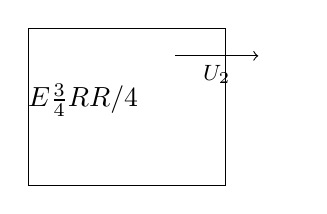
\begin{tikzpicture}[font=\footnotesize]
	\draw (0,-1)rectangle(2.5,1);
	% \draw (2,-1)--++(0,2);
	\pileL{}{$E$};
	\resistanceV{shift={(2.5,0)}}{$\frac34 R$};
	% \resistanceV{shift={(3,0)}}{$3R$};
	\resistanceH{shift={(1,1)}}{$R/4$};
	\draw[shift={(2.5,0)},->](10pt,-15pt)--++(0,30pt)node[midway,right]{$U_1$};
	\draw[shift={(1,1)},->](-15pt,-10pt)--++(30pt,0)node[midway,below]{$U_2$};
\end{tikzpicture}
	\end{center}
	On reconnaît un diviseur de tension. La formule du diviseur donne $U_1=E\times \frac{\frac34 R}{\frac14 R+\frac34 R}=\frac34 E$. 
\end{corrigeNewpage}

% ^^^^^^^^^^^^^^^^^^^^^^^^^^^^^^^^^^^^^^ %
%               Question                 %
% ^^^^^^^^^^^^^^^^^^^^^^^^^^^^^^^^^^^^^^ %

\begin{enonce}
Faire la même chose pour $U_2$.
\end{enonce}

\reponse{$-\frac{E}{4}$}

\begin{corrige}
	Là encore on peut utiliser la formule du diviseur de tension en faisant attention à l'orientation : 
	\[
		-U_2=E\times\frac{\frac14 R}{\frac14 R+\frac34 R}
		\quad\text{soit}\quad
		U_2=-\frac{E}{4}.
	\]
	\textbf{Remarque} : on peut aussi obtenir $U_2$ à l'aide de la loi des mailles : $E+U_2-U_1=0$ avec $U_1=\frac34 E$.
\end{corrige}

% ************************************** %

% =============================================================================== %
\finEntrainement
% =============================================================================== %




% ********************************************************************* %
%                           ENTRAÎNEMENT                                % 
% ********************************************************************* %
% ================ Métadonnées sur l'entraînement ===================== %

\titreEntrainementFacultatif	{Exercice de synthèse II}
\hauteurLargeurCadreReponse		{7mm}{15mm}
\dureeResolutionFacultative		{3} % 1, 2, 3 ou 4
\typeEntrainement				{} % Newton ou QCM ou AN ou vide (exercice "normal")
\nombreColonnesQuestions		{1} % vide, 1, 2, 3, etc.
\avecPlusieursQuestions			{Y} % Y ou N
\initialisationEntrainement
% ===================================================================== %

\begin{center}
\subimport{_images/}{fiche_ELC01_diviseur_courant1_CBD_v3.tex}
\end{center}

% =============================================================================== %
\debutEntrainement
% =============================================================================== %

% ^^^^^^^^^^^^^^^^^^^^^^^^^^^^^^^^^^^^^^ %
%               Question                 %
% ^^^^^^^^^^^^^^^^^^^^^^^^^^^^^^^^^^^^^^ %

\begin{enonce}
	Après avoir simplifié le circuit, calculer $i$ en fonction de $E$ et $R$
\end{enonce}

\reponse{$\frac{3E}{8R}$}

\begin{corrige}
	Remplaçons l'association $(2R\parallel R)$ par un conducteur de résistance $R_\text{eq}=\frac{2R\times R}{2R+R}=\frac23 R$. On obtient le circuit à une maille suivant :
	\begin{center}
	%\subimport{_images/}{fiche_ELC01_diviseur_courant1_rep_JRL_v2.tex}
	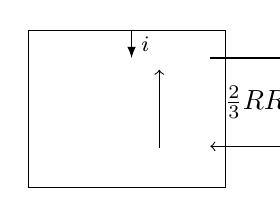
\begin{tikzpicture}[
	font=\footnotesize,
	]
	\draw (0,-1)rectangle (-2.5,1);	
	\resistanceV{shift={(-2.5,0)}}{$\frac23 R$};
	\resistanceH{shift={(-1,1)}}{$R$};
	\resistanceH{shift={(-1,-1)}}{$R$};
	\FEMVR{shift={(0,0)}}{$E$};
	\draw[-latex,shift={(0,.5)}](0,-5pt)--++(0,10pt)node[midway,right]{$i$};
	\draw[-latex,shift={(-2.5,1)}](0,0)--++(0,-10pt)node[midway,right]{$i$};
	\draw[->,shift={(-1,10mm-10pt)}](-.5,0)--++(1,0);
	\draw[->,shift={(-1,-10mm+15pt)}](.5,0)--++(-1,0);
	\draw[->,shift={(-25mm+10pt,0)}](0,-.5)--++(0,1);
\end{tikzpicture}

	\end{center}
	La loi des mailles donne alors $E-Ri-\frac23 Ri-Ri=0$, d'où $i=\frac38 \frac{E}{R}$.
\end{corrige}

% ^^^^^^^^^^^^^^^^^^^^^^^^^^^^^^^^^^^^^^ %
%               Question                 %
% ^^^^^^^^^^^^^^^^^^^^^^^^^^^^^^^^^^^^^^ %

\begin{enonce}
	En déduire $i_1$ à partir de la formule du diviseur de courant
\end{enonce}

\reponse{$\frac{E}{4R}$}

\begin{corrige}
	La formule du diviseur donne 
	\[
		i_1=\frac{1/R}{1/R+1/(2R)}\times i=\frac23 i= \frac{E}{4R}.
	\]
\end{corrige}

% ^^^^^^^^^^^^^^^^^^^^^^^^^^^^^^^^^^^^^^ %
%               Question                 %
% ^^^^^^^^^^^^^^^^^^^^^^^^^^^^^^^^^^^^^^ %

\begin{enonce}
	En déduire $i_2$
\end{enonce}

\reponse{$-\frac{E}{8R}$}

\begin{corrige} 
	Le plus simple consiste à utiliser la loi des n\oe uds : $i+i_2=i_1$ ce qui donne $i_2=i_1-i=-\frac{E}{8R}$.
	
	On peut aussi utiliser la formule du diviseur de courant en faisant attention à l'orientation des courants : 
	\[
		-i_2=\frac{1/(2R)}{1/R+1/(2R)}\times i=\frac13 i=\frac{E}{8R}.		
	\]
\end{corrige}

% ************************************** %

% =============================================================================== %
\finEntrainement














% ---------------------------------------------------------------------------- %
%                       Affichage des réponses mélangées                       %
% ---------------------------------------------------------------------------- %
\afficheReponsesMelangees
% ---------------------------------------------------------------------------- %

%%%%%%%%%%%%%%%%%%%%%%%%%%%%%%%%%%%%%%%%%%%%%%%%%%%%%%%%%%%%%%%%%%%%%%%%%%%%%%%%%%%%%%%%%%%%%%
\finFicheEntrainement                                                                        %
%%%%%%%%%%%%%%%%%%%%%%%%%%%%%%%%%%%%%%%%%%%%%%%%%%%%%%%%%%%%%%%%%%%%%%%%%%%%%%%%%%%%%%%%%%%%%%


% ======================================================= % 
% ============== Gestion de la compilation ============== %
% ======================================================= % 
\ifdefined\mainIsLoaded\else
\printReponsesEtCorriges
\end{document}\fi
% ======================================================= % 
% ======================================================= % 





















% % ********************************************************************* %
% %                           ENTRAÎNEMENT                                %
% % ********************************************************************* %
% % ================ Métadonnées sur l'entraînement ===================== %
%
% \titreEntrainementFacultatif	{Un entraînement fondamental}
% \hauteurLargeurCadreReponse		{8mm}{7cm}
% \dureeResolutionFacultative		{1} % 1, 2, 3 ou 4
% \typeEntrainement				{AN} % Newton ou QCM ou AN ou vide (exercice "normal")
% \nombreColonnesQuestions		{3} % vide, 1, 2, 3, etc.
% \avecPlusieursQuestions			{Y} % Y ou N
% \initialisationEntrainement
% % ===================================================================== %
%
% Les trois dipôles électriques suivants sont équivalents à un conducteur ohmique. Calculer leur résistance équivalente.
% \begin{center}
% \subimport{_images/}{fiche_ELCO1_Req1_JRL_v1.tex}
% \end{center}
%
% % =============================================================================== %
% \debutEntrainement
% % =============================================================================== %
%
% % ^^^^^^^^^^^^^^^^^^^^^^^^^^^^^^^^^^^^^^ %
% %               Question                 %
% % ^^^^^^^^^^^^^^^^^^^^^^^^^^^^^^^^^^^^^^ %
%
% \begin{enonce}
% Pour le dipôle 1.
% \end{enonce}
%
% \reponse{$1$}
%
% %\begin{corrige}
% %\end{corrige}
%
% % ************************************** %
% % ^^^^^^^^^^^^^^^^^^^^^^^^^^^^^^^^^^^^^^ %
% %               Question                 %
% % ^^^^^^^^^^^^^^^^^^^^^^^^^^^^^^^^^^^^^^ %
%
% \begin{enonce}
% Pour le dipôle 2.
% \end{enonce}
%
% \reponse{$1$}
%
% %\begin{corrige}
% %\end{corrige}
%
% % ************************************** %
% % ^^^^^^^^^^^^^^^^^^^^^^^^^^^^^^^^^^^^^^ %
% %               Question                 %
% % ^^^^^^^^^^^^^^^^^^^^^^^^^^^^^^^^^^^^^^ %
%
% \begin{enonce}
% Pour le dipôle 3.
% \end{enonce}
%
% \reponse{$1$}
%
% %\begin{corrige}
% %\end{corrige}
%
% % ************************************** %
%
% % =============================================================================== %
% \finEntrainement
% % =============================================================================== %

% % ********************************************************************* %
% %                           ENTRAÎNEMENT                                %
% % ********************************************************************* %
% % ================ Métadonnées sur l'entraînement ===================== %
% \titreEntrainementFacultatif	{Allume le voltmètre}
% \hauteurLargeurCadreReponse		{8mm}{1.5cm}
% \dureeResolutionFacultative		{1} % 1, 2, 3 ou 4
% \typeEntrainement				{QCM} % Newton ou QCM ou AN ou vide (exercice "normal")
% \nombreColonnesQuestions		{1} % vide, 1, 2, 3, etc.
% \avecPlusieursQuestions			{N} % Y ou N
% \initialisationEntrainement
% % ===================================================================== %
% % mmmmmmmmmmmmmmmmmmmmmmmmmmmmmmmmmmmmmmmmmmmmmmmmmmmmmmmmm %
% % 		  Insertion d'une image en regard d'un texte
% % mmmmmmmmmmmmmmmmmmmmmmmmmmmmmmmmmmmmmmmmmmmmmmmmmmmmmmmmm %
% % --------------------------------------------------------- %
% \pourcentageDeLaPartieAGauche   {0.5}
% % --------------------------------------------------------- %
% %                                                           %
% % -------------------- Partie à gauche -------------------- %
% %                                                           %
%                                 \initialisationPartieGauche %
% %                                                           %
% %                                                           %
% Une pile alimente une ampoule portant les indications (\np[V]{12}-\np[A]{0.1}).
%
% \smallskip
%
% Qu'indique le voltmètre lorsque l'interrupteur K est ouvert ?
% % --------------------------------------------------------- %
% %                                                           %
% % -------------------- Partie à droite -------------------- %
% %                                                           %
%                                 \initialisationPartieDroite %
% %                                                           %
% %                                                           %
% \begin{center}
% \subimport{_images/}{fiche_ELC01_voltmetre_JRL_v1.tex}
% \end{center}
% % --------------------------------------------------------- %
%                                \finalisationDuPartageDePage %
% % --------------------------------------------------------- %
%
%
% % =============================================================================== %
% \debutEntrainement
% % =============================================================================== %
%
%
% % ^^^^^^^^^^^^^^^^^^^^^^^^^^^^^^^^^^^^^^ %
% %               Question                 %
% % ^^^^^^^^^^^^^^^^^^^^^^^^^^^^^^^^^^^^^^ %
% \begin{enonce}
% 	\begin{listeQCM2Colonnes}
% 	\item \np[V]{0}
% 	\item \np[V]{12}
% 	\item ERREUR
% 	\item \np[V]{4.5}
% 	\end{listeQCM2Colonnes}
%
% \end{enonce}
%
% \reponse{\reponseC{}}
%
% \begin{corrige}
% 	Bla bla
% \end{corrige}
%
% % ************************************** %
%
% % =============================================================================== %
% \finEntrainement
% % =============================================================================== %
